% Teilaufgabe 2

\newpage
\section{Konstruktive Interferenz senkrecht zu Medium}
\label{sec:interferenz}
\begin{center}
	\captionsetup{type=figure}
	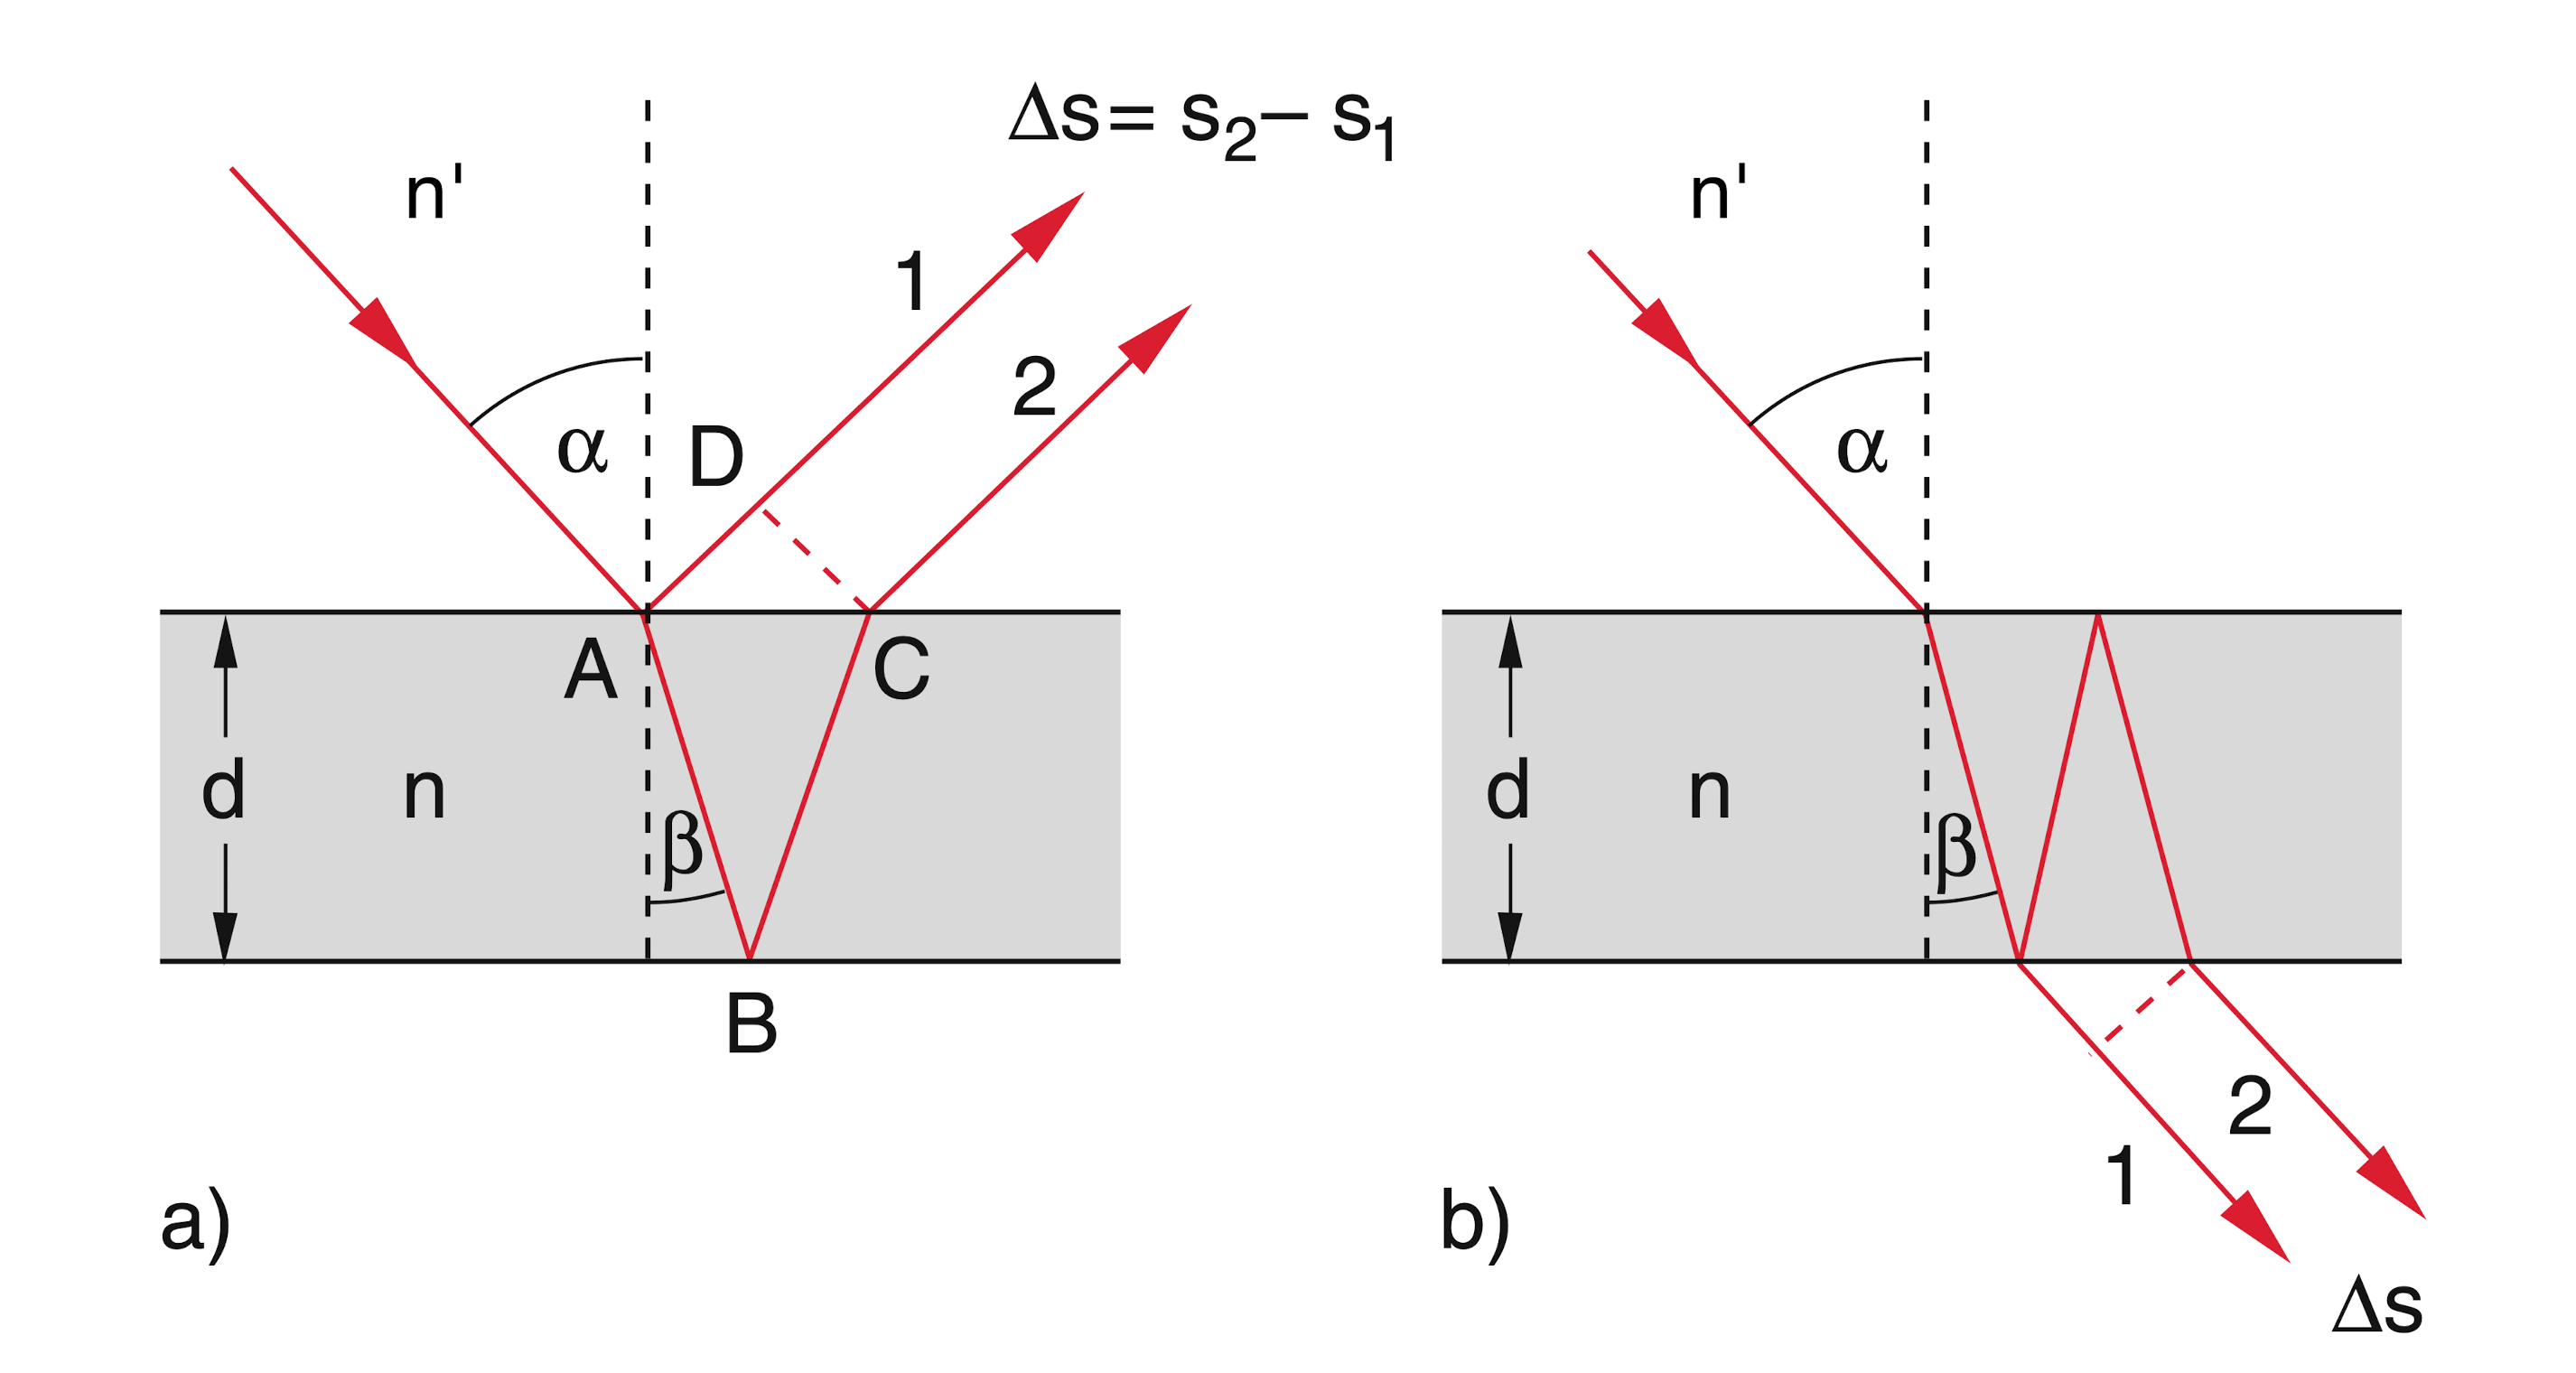
\includegraphics[width=0.75\textwidth]{Konstruktive-Interferenz.png}
	\captionof{figure}{
		Brechung an einer planparallelen Platte mit allgemeinen Einfallswinkel $\alpha$\\
		\textbf{a)} Ebene Welle wird am Medium reflektiert\\
		\textbf{b)} Ebene Welle wird im Medium transmittiert \cite{DemtroederOptik}}
	\label{fig:interferenz}
\end{center}
Es wird ein Substrat (Medium) mit endlicher Dicke $d$ und Brechungsindex $n$ untersucht. Außerhalb des Mediums (Brechungsindex $n'$) trifft ein ebene Welle mit Wellenlänge $\lambda$ unter dem Winkel $\alpha$ (Winkel zwischen Lot und Lichtstrahl) auf das Medium und wird ein Teil der Welle reflektiert (Teilwelle 1) [Abb. \ref{fig:interferenz} a)] und der andere Teil der Welle gebrochen Teilwelle 2 [Abb. \ref{fig:interferenz} b)]. Die gebrochene Welle wird an der unteren Begrenzungsschicht erneut reflektiert, tritt parallel zur Teilwelle 1 durch die obere Grenzfläche und überlagert sich dieser Teilwelle.\bigskip

Um Interferenz einem optischen Medium zu berechnen wird zu erst der Gangunterschied $\Delta s$ benötigt.
Dieser ist definiert als der Wegunterschied zwischen Teilwelle 1 und Teilwelle 2: 
\begin{gather}
	\begin{aligned}
		\Delta s &= s_2 - s_1 = n(\overline{AB} + \overline{BC}) - n'(\overline{AD}) \\ 
		\xrightarrow[\mathrm{Abb.}~ \ref{fig:interferenz} \mathrm{a)}]{\mathrm{Trigonometrie}} \Delta s &= \frac{2nd}{\cos\beta} + 2n'd\tan\beta\sin\alpha
	\end{aligned}
	\label{eq:gangunterschiedAllg} 
\end{gather}
Gleichung \ref{eq:gangunterschiedAllg} gilt auch für die transmittierte Welle [Abb. \ref{fig:interferenz} b)], was aber hier nicht explizit gezeigt wird. Wenn nun die ebene Welle senkrecht auf das Substrat fällt ($\alpha = 0$) folgt aus dem Snellius`schen Brechungsgesetz:
\begin{gather}
	n'\sin\alpha=n\sin\beta \xrightarrow{\alpha=0} n\sin\beta = 0 \Rightarrow \boxed{\beta = 0}
	\label{eq:brechung}
\end{gather}
Setzt man nun das Ergebnis von Gleichung \ref{eq:brechung} in die Gleichung für den Gangunterschied \ref{eq:gangunterschiedAllg} folgt:
\begin{gather}
	\xrightarrow[\beta = 0]{\alpha = 0} \boxed{\Delta s = 2nd}
	\label{eq:gangunterschied}
\end{gather}\bigskip

Als nächstes wird er Phasenunterschied $\Delta \varphi$ betrachtet, der wie folgt definiert ist:
\begin{gather}
	\begin{aligned}
		 \Delta \varphi &= \frac{2\pi}{\lambda}\Delta s - \pi &\mathrm{(reflektierte~Welle)}\\
		 \Delta \varphi &= \frac{2\pi}{\lambda}\Delta s &\mathrm{(transmittierte~Welle)}
	\end{aligned}
	\label{eq:phase}
\end{gather}
Hierbei ist zu beachten, dass die reflektierte Welle eine Phasensprung um $\pi$ aufweist. Zusätzlich gilt für konstruktive Interferenz die Bedingung:
\begin{gather}
	\boxed{\Delta \varphi = 2\pi m;~m \in \mathbb{N}}
	\label{eq:interferenz}
\end{gather}
wobei $m$ die Beugungsordnung der Interferenz ist. Setzt man nun den Gangunterschied aus Gleichung \ref{eq:gangunterschied} und die Bedingung für konstruktive Interferenz (Gleichung \ref{eq:interferenz}) in Gleichung \ref{eq:phase} ein und löst nach der Wellenlänge $\lambda$ auf, erhält man: \cite{DemtroederOptik}
\begin{gather}
	\boxed{
	\begin{aligned}
		 \lambda &= \frac{2nd}{m + 1/2} &;~m \in \mathbb{N} ~&\mathrm{(reflektierte~Welle)}\\
		 \lambda &= \frac{2nd}{m}       &;~m \in \mathbb{N} ~&\mathrm{(transmittierte~Welle)}
	\end{aligned}
	}
	\label{eq:wavelength}
\end{gather}